\documentclass[main.tex]{subfiles}


\begin{document}

\begingroup

\renewcommand{\cleardoublepage}{}

\renewcommand{\clearpage}{}

\chapter{Perception Function Documentation}

\chapterauthor{Leonidas Paniago}
		\section{rs\_perception}

			\subsection{Pipeline: hsrb\_1ms}

The main pipeline for detecting and identifying objects with RoboSherlock consists of following annotators:  
\begin{itemize}
	\item CollectionReader : Takes care of the camera input
	\item ImagePreprocessor : Implements image filters  
	\item SuturoRegionFilter : Removes all points that are not in the defined regions 
	\item NormalEstimator : Estimate surface normals in a PointCloud 
	\item PlaneAnnotator : Finds a plane in the current scene and saves it into the CAS.
	\item PointCloudClusterExtractor : Extracts all points that are found in the PointCloud that are perpendicular to the plane 
	\item ClusterColorHistogramCalculator : Calculate the individual color quantity in relation to all colors in the cluster   
	\item Cluster3DGeometryAnnotator : Extracts basic attributes of the cluster, like initial pose, semantic size and 3D bounding box 
	\item PrimitiveShapeAnnotator : Annotates basic shapes to the cluster
	\item RegionAnnotator : Annotates the name of the region that surrounds the detected object
	\item CaffeAnnotator : Deep learning method for Object recognition based on pre recorded images 
	\item KnnAnnotator : Uses K-Nearest-Neighbor for the classification of objects 
\end{itemize}

Each annotator contains changeable variables that enable customization to the given tasks, for most of time we used the default settings. 
RoboSherlock pipeline works sequential meaning any change to the order can change the result. Some of the annotators are essential for the pipeline to work, like the CollectionReader. 
Furthermore for any new annotator created, need to consideration where to put it.\\
 The following Pictures are an example of the RoboSherlock pipeline output :  \\
%Bild Hinzufügen 

\begin{figure}[H]
     \begin{center}
%
        \subfigure[2D-ImagePreProcessor]{%
            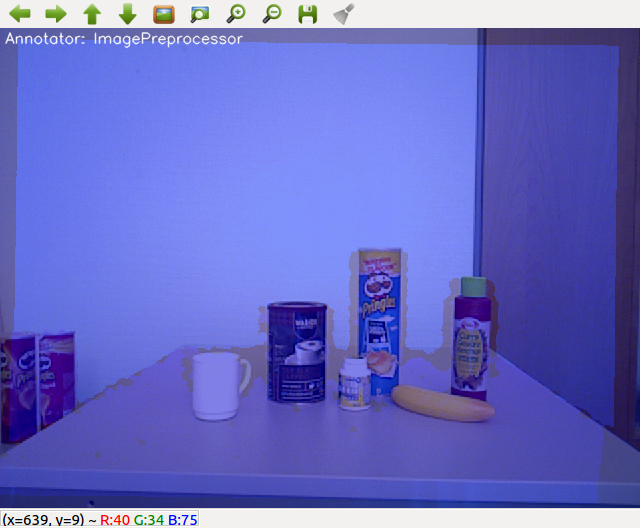
\includegraphics[width=0.5\textwidth]{pictures/2d/ImagePreProcessor.png}
        }%
        \subfigure[3D-RegionFilter]{%
           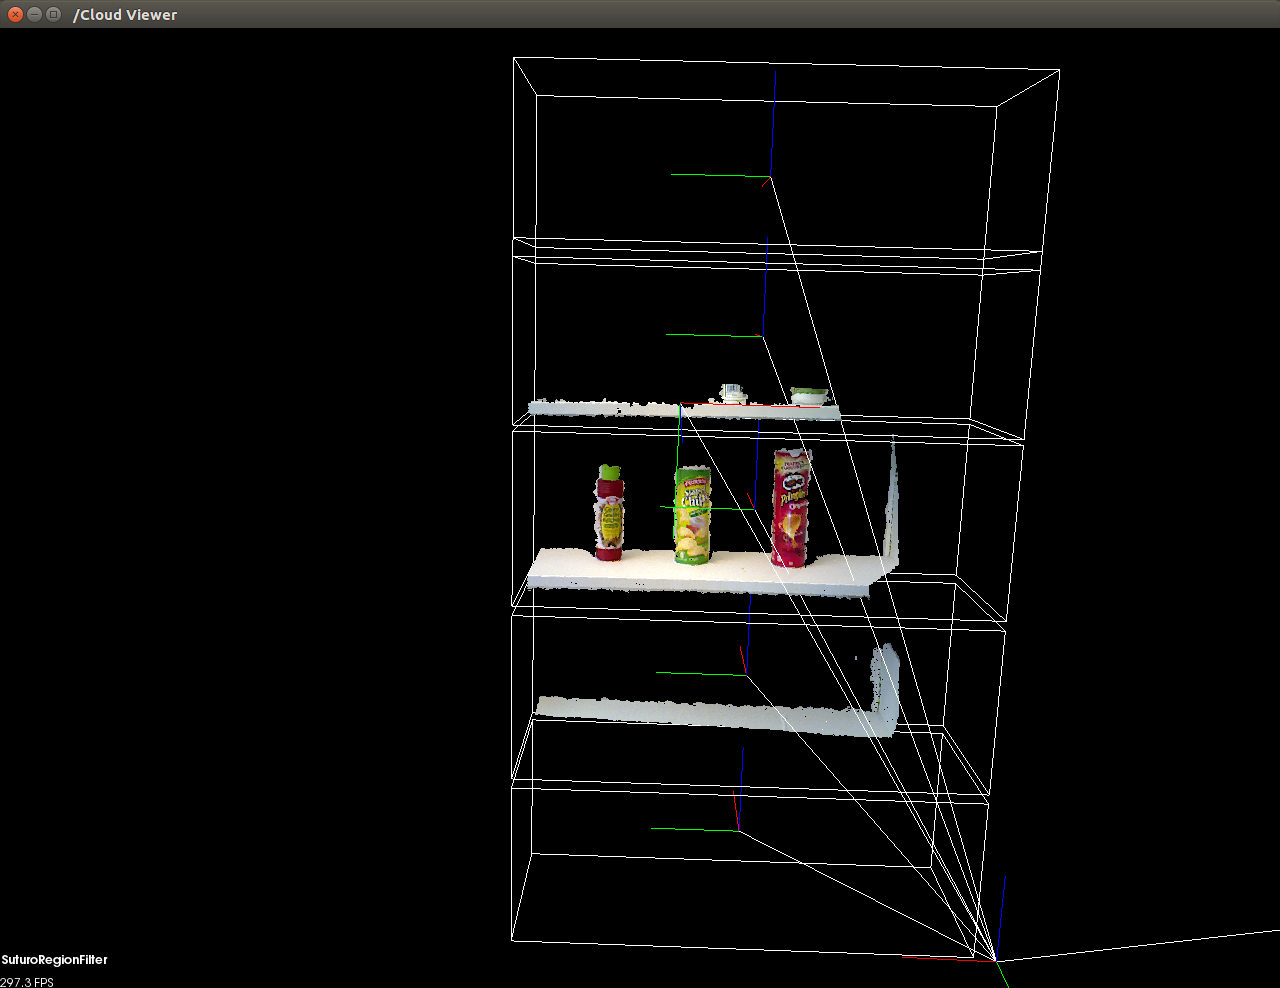
\includegraphics[width=0.5\textwidth]{pictures/pcl/RegionFilter.png}
        }\\ %  ------- End of the first row ----------------------%
        \subfigure[2D-NormalEstimator]{%
            \includegraphics[width=0.5\textwidth]{pictures/2d/NormalEstimator.png}
        }%
        \subfigure[3D-NormalEstimator]{%
           \includegraphics[width=0.5\textwidth]{pictures/pcl/NormalEstimator.png}
        }%
%
    \end{center}
\end{figure}

\begin{figure}[H]
     \begin{center}
%
        \subfigure[2D-PlaneAnnotator]{%
            \includegraphics[width=0.5\textwidth]{pictures/2d/PlaneAnnotator.png}
        }%
        \subfigure[3D-RegionFilter]{%
           \includegraphics[width=0.5\textwidth]{pictures/pcl/PlaneAnnotator.png}
        }\\ %  ------- End of the first row ----------------------%
        \subfigure[2D-PointCloudClusterExtractor]{%
            \includegraphics[width=0.5\textwidth]{pictures/2d/PointCloudClusterExtractor.png}
        }%
        \subfigure[3D-PointCloudClusterExtractor]{%
            \includegraphics[width=0.5\textwidth]{pictures/pcl/PointCloudClusterExtractor.png}
        }%
%
    \end{center}
\end{figure}

\begin{figure}[H]
     \begin{center}
%
        \subfigure[2D-ClusterColorHistogramAnnotator]{%
            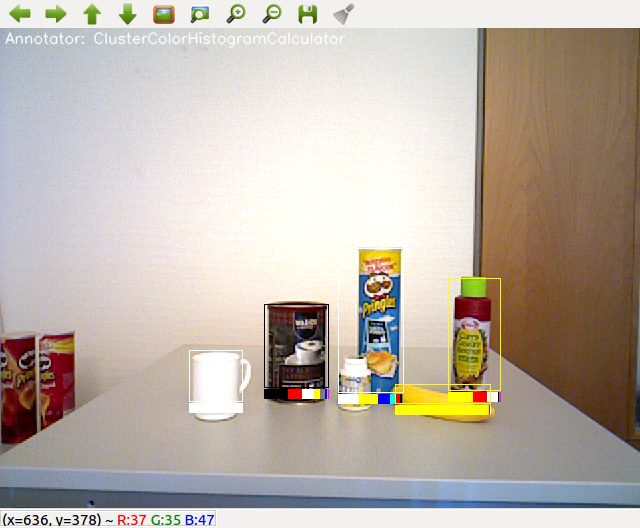
\includegraphics[width=0.5\textwidth]{pictures/2d/ClusterColorHistogramAnnotator.png}
        }%
        \subfigure[2D-Cluster3DGeometryAnnotator]{%
          \includegraphics[width=0.5\textwidth]{pictures/2d/Cluster3DGeometryAnnotator.png}
        }\\ %  ------- End of the first row ----------------------%
        \subfigure[3D-Cluster3DGeometryAnnotator]{%
            \includegraphics[width=0.5\textwidth]{pictures/pcl/Cluster3DGeometryAnnotator.png}
        }%
%
    \end{center}
\end{figure}

\begin{figure}[H]
     \begin{center}
%
         \subfigure[2D-PrimitiveShapeAnnotator]{%
           \includegraphics[width=0.5\textwidth]{pictures/2d/PrimitiveShapeAnnotator.png}
        }%
        \subfigure[2D-SuturoShapeAnnotator]{%
           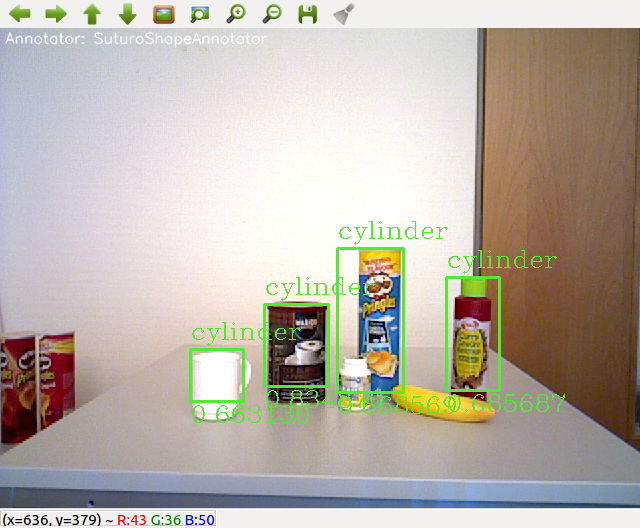
\includegraphics[width=0.5\textwidth]{pictures/2d/SuturoShapeAnnotator.png}
        }\\ %  ------- End of the first row ----------------------%
         \subfigure[3D-PrimitiveShapeAnnotator]{%
            \includegraphics[width=0.5\textwidth]{pictures/pcl/PrimitiveShapeAnnotator.png}
        }%
        \subfigure[2D-KnnAnnotator]{%
            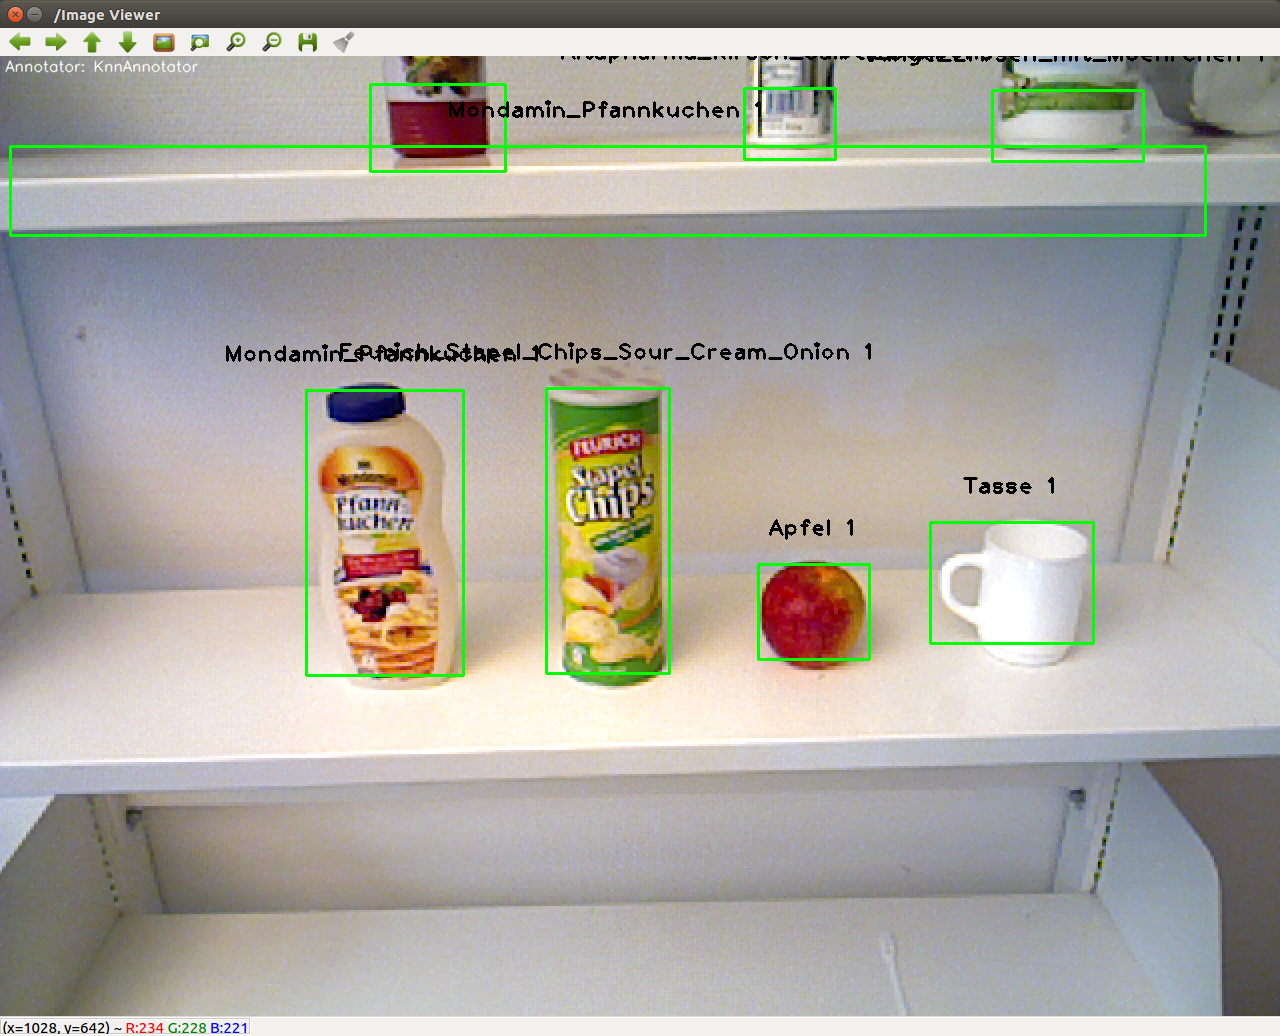
\includegraphics[width=0.5\textwidth]{pictures/2d/KnnAnnotator.png}
        }%
%
    \end{center}
\end{figure}

			\subsection{Pipeline: hsrb\_planes} 
This pipeline is used to detect a shelf door. We try to find a plane that is parallel to the camera.
\begin{itemize}
	\item CollectionReader : Takes care of the camera input
	\item ImagePreprocessor : Implements image filters  
	\item PointCloudFilter : Filters points out of the cloud that are not in the range of the given parameters for X, Y and Z axes
	\item NormalEstimator : Estimate surface normal's in a PointCloud 
	\item PlaneAnnotator : Finds a plane in the current scene and saves it into the CAS.
	\item PointCloudClusterExtractor : Extracts all points that are found in the PointCloud that are perpendicular to the plane 
\end{itemize}

			\subsection{Pipeline: storage\_suturo} 
Pipeline for storing the actual scene in MongoDB, all saved scenes can be replayed for testing without the HSR and have the same functionality. 
\begin{itemize}
	\item CollectionReader : Takes care of the camera input
	\item ImagePreprocessor : Implements image filters 
	\item StorageWriterSuturo :  Store set topics in MongoDB
\end{itemize}

		\section{actionserver}

			\subsection{ExtractObjectInfoClient}
Call ExtractObjectInfoServer and wait until the result arrives or the time out runs out. Region can be set to limit the perception of objects to a specific region, if default is set the RegionFilter will be disabled. 

			\subsection{ExtractObjectInfoServer}
Receives a goal from ExtractObjectInfoClient and then SuturoProcessManager, Checks for result and publishes it under perception\_actionserver/result 

			\subsection{ExtractPlaneInfoClient}
Call ExtractPlaneInfoServer and wait until the result arrives or the time out runs out. This client has no additional parameters.

			\subsection{ExtractPlaneInfoServer}
Receives a goal from ExtractPlaneInfoClient and pass on to SuturoPrecessManager, Checks for result and publishes it under perception\_actionserver\_plane/result.

			\subsection{perception\_server}
Launch ExtractObjectInfoServe and ExtractPlaneInfoServer no other Functionality.

%		\section{rs\_hsrb\_perception}
%rs\_hsrb\_perception is package from the last Suturo group. All changes are made to the new sub Branch suturo20.

%			\subsection{SuturoProcessManager}
%Annotator based on RSProcessManager. Starts different Robosherlock pipelines based on witch Server makes the Call.  Each server use the same run method with different arguments. 

		\section{rs\_turn\_table}
rs\_turn\_table is package from the last Suturo group.There was no big changes to the core code, only small situational changes not implemented on the master. 
This package is mainly for Image recording, All recorded images will then be used for Object recognition.  
			\subsection{Pipeline: estimate\_plane}
\begin{itemize}
	\item CollectionReader : Takes care of the Camera  Input
	\item ImagePreprocessor : Create missing Images and implement Image Filters  
	\item PointCloudFilter : Filter Points that are over set limitations like size and depth
	\item PlaneAnnotator : Finds a plane and save it to a file 
\end{itemize}
This Pipeline will save all visible planes, they are callable again. The best way to get a clean plane is to set the Limits on PointCloudFilter by hand. It is desirable that only one plane is visible. 

			\subsection{Pipeline: save\_images}
\begin{itemize}
	\item CollectionReader : Takes care of the Camera  Input
	\item ImagePreprocessor : Create missing Images and implement Image Filters  
	\item PointCloudFilter : Filter Points that are over set Limitations like Size and Depht
	\item PlaneAnnotator : Use saved plane in which the search location for Objects is set
	\item PointCloudClusterExtractor : Extract all Points found in the PointCloud that are perpendicular to the Plane 
	\item SaveClusterCloudsAndImages : Save Information about the Cluster to a file 
\end{itemize}
Uses the saved Plane and take periodic Images from Objects on the plane, if there is more that one Cluster visible the Annotator will not trigger the Save process.

\section{classificationEvaluation Package}
\chapterauthor{Jan-Frederik Stock}

The classificationEvaluation package is used to save and display the classificationresults of the perceptionpipeline. The results can be saved in a markdown table and/or be displayed as a scatterplot. It consists mainly of the rsClassificationEvaluator.py pythonscript. Here, the class ResultActionClient is implemented, which serves as an actionclient for the perception object info actionserver.\\

\subsection{The ResultActionClient class}
The class provides the following methods:

\begin{itemize}
\item 
sendGoal(self)\\
This method is used to send a goal to the ExtractObjectInfoServer and thus triggering the perceptionpipeline.

\item saveResult(self, result)\\
This method saves the actionresult, which is the classification, in a field of the class.

\item saveToMd(self, algorithm)\\
This method saves the collected classifcationresults in a markdown table. If a markdown file with the name "evaluation.md" is found in the directory the script is executed in, the results are appended to it, otherwise the file is created.

\item plotResult(self)\\
The method plots the collected results using the scatterplotfunction from matplotlib.

\subsection{Main method}
The main method tries to create an instance of the resultActionClient class, does some i/o with the user, sets the parameters for the resultActionClass and then triggers the action. It also uses the provided methods to save the results to a markdown file and plot them.

\section{Feature Extraction Tools}
The tools directory in the featureExtraction package contains the two bash scripts make\_split\_from\_directory.sh and make\_split\_list\_from\_directory.sh.

\subsection{make\_split\_from\_directory.sh} 
This bash script can be used to create a split yaml-file which is required to perform feature extraction with the rs\_addons package. To use it, one has to place the file in the parentdirectory of the directory, in which the folders with the recorded images are stored. When being executed, the script asks for a filename and the name of the directory out of which the yaml-file will be created. It then creates the yaml-file using the directorynames of the imagedirectories as classnames.

\subsection{make\_list\_from\_directory.sh}
This bash script does nearly the same thing as the make\_split\_from\_directory.sh, except that it does not create a splitfile but a list of the classnames. This is required by the classifing annotator and has to be pasted into the annotators yaml-file. The comma after the last classname in the list has to be removed manually.

\section{calculateConfidence in RSKNN.cpp}
In the RSKNN.cpp, implementing KNN-classification in the rs\_addons package, the following method was added:

\begin{lstlisting}
double RSKNN::calculateConfidence(double classificationResult, cv::Mat neighborResponses)
\end{lstlisting}

It calculates the classification confidence for the KNN-classification by dividing the number of neighbours belonging to the result class, by the total number of visited neighbours. 

\end{itemize}


\section{rs\_hsrb\_perception Package}
\chapterauthor{Evan Kapitzke}

The rs\_hsrb\_perception package was created in the Suturo Master-project. The package implements an RoboSherlock process manager, namely SuturoProcessManager. Additionally, it contains modified annotators to annotate regions.

\subsection{RegionAnnotator}
\begin{itemize}
\item TyErrorId process(tcas, res\_spec)\\
Iterates through the clusters that are currently saved in the CAS and annotates the region in which their are present based on the cluster pose.
This method only got changed in order to work with the RoboSherlock master.
\end{itemize}

\subsection{SaveClusterCloudsAndImages}
Currently not used.

\subsection{SuturoClassifier}
Currently not used.

\subsection{SuturoProcessManager}
\begin{itemize}
\item setup()\\
Creates the ressource manager and instantiates the region vector.

\item init(pipeline)\\
Initializes the given pipeline (aggregate analysis engine YAML descriptor) and starts the visualizer.
This method got changed in order to allow the visualization of the pipeline.

\item run(args, detectionData)\\
Executes the initialized pipeline once with the given arguments and saves the result in detectionData.
This method now checks for the region "robocup\_default" and disables the region filter to perceive objects that can not be found
in a region. For example, a pringles dose that is placed on the ground.

\item has\_vertical\_plane()\\
Returns true if the current CAS contains a vertical plane.

\item getClusterFeatures(cluster, data)\\
Extracts the annotations of the given cluster and generates an ObjectDetectionData object. 
This object will be added to the data pointer. makeObjectDetectionData(...) from suturo\_conversion is used.
Currently only one KnnAnnotator (for known objects) is used to determine the class label of an object.

\item visControlCallback(req, res)\\
Callback for navigation through the different annotation previews in the visualization window.
\end{itemize}

\subsection{SuturoRegionFilter}
Adapted region filter from RoboSherlock.

\begin{itemize}
\item reconfigure()\\
Reconfigures the annotator to disable / enable its functionality without restarting the pipeline or removing it.
\end{itemize}

\subsection{suturo\_conversion}
Implements template functions to convert from and to PoseStamped objects.
Following functions got changed:

\begin{itemize}
\item decode\_shape(shapes)\\
Converts the result of the PrimitiveShapeAnnotator to match the required shape format in the ObjectDetectionData object.

\item makeObjectDetectionData(pose, geometry, shape, objClass, confidence, c, odd)\\
Combines the given parameters to an ObjectDetectionData message.
\end{itemize}

\endgroup
\end{document}
